\label{chap:linguistic_persuasion}

\section{\statusgreen Introduction}
\label{sec:lp_intro}

% what (orientation)
In this chapter, we add our second ingredient: persuasion. We intend persuasion as a general umbrella that encompasses several phenomena where the writer of a piece of text is trying to persuade the reader of a certain point of view.

% why (rationale)
From the last chapter~\ref{chap:common_ground_search}, we concluded with the need to understand how specific terms are used to persuade the reader. We are able to extract terms that have been changed in related articles, but we want to characterise them quantitatively along some dimensions that can describe or are related to persuasion.

For this reason, this chapter investigates the \emph{linguistic proxies of persuasion}, in other words how the persuasion manifests itself on the textual/linguistical surface.

% aim
Our motivation is to analyse whether the terms that change between multiple articles/sentences are correlated with the linguistic proxies of persuasion.

The Research Questions we want to answer are: 
\begin{enumerate}
    \item What do writers use to persuade the reader?
    \item Is there a link between the parts that are different and persuasion proxies (propaganda/loaded language)?
    \item Which are the possible indicators of these differences? 
\end{enumerate}


% method
% strong/loaded language: using sentiment analysis tools 
% 18 techniques of propaganda

% Experiment together with common ground search
To answer these research questions, we carry the following experiment:

We take into study the terms that change between articles and we analyse whether there exist some persuasion proxies that indicate something about the changes in the sentences.

This is implemented according to the following pipeline:
\begin{enumerate}
    \item Analysis from Chapter~\ref{chap:common_ground_search}: extracts the words that are changed between similar sentences of similar articles
    \item Extraction of different proxies (sentiment, propaganda, persuasion) on the sentences (described in the next Section~\ref{sec:lp_proxies}
    \item Analysis of the relationship between these proxies and the changes in the sentences (described in Section~\ref{sec:lp_relationship})
\end{enumerate}


% findings
We discover that sentiment itself is not very precise to indicate the persuasion, while the initial methods for fine-grained propaganda detection seem to be more promising. For this reason, we mainly use propaganda for the experiments of the following chapters. 

Our findings from this chapter include:
\begin{enumerate}
    \item The relationship between the changed terms and propaganda language is not very clear: different parts are not always loaded with loaded language or propaganda. A lot of changes are not meaningful in terms of propaganda: linguistic variance.
    \item Removing propaganda and/or sentiment from articles makes related articles slightly easier to cluster correctly.
\end{enumerate}

% interpretation

% TODO: Interpretation? Or just pointers to next sections
The next sections are organised as follows. Section~\ref{sec:lp_proxies} contains some proxies that we identifed being related to persuasion. We present there what they are able to detect on our datasets (stage 2 of the pipeline above described). Then Section~\ref{sec:lp_relationship} contains two experiments aimed at understanding the relationship between these proxies and the words changed (stage 3 of the pipeline).

\section{Different Proxies}
\label{sec:lp_proxies}

% TODO preamble to different proxies: sentiment, propaganda, populism, ...

From all the different methods and approaches described in Chapter~\ref{sec:lit_propaganda}\tododefault{check ref}, in this section, we are using a round of tools that aims at detecting phenomena related to persuasion and manipulation and do that at the word-level.
In other words, we are using several proxies that we assume to be related to persuasion: sentiment (subjectivity), propaganda and populism.
And we require to be able to work at the word-level, because our end goal is to study the relationship between them and the variations across the articles (as will be seen in Section~\ref{sec:lp_relationship}). Only having a score for the whole article or for a whole sentence is not helpful, because we need word-level information. We are analysing word substitutions.

\subsection{Sentiment detection}

First of all, we start with some sentiment detection. It is known that persuasion is related to an emotional response from the reader/listener, being related to emotions~\citep{rocklage2018persuasion,petty2015emotion,desteno2004discrete} and to sentiment~\citep{gatti2014sentiment}.
While computational approaches to detect emotions (usually quantified across the 5-big emotions) exist, the computational tools available for sentiment detection are more numerous and more common. The main disadvantage of only using sentiment detection instead of emotions is that it usually gives an output on 1 or 2 axes: valence (positive or negative) and strength (from neutral to strong). But for an initial analysis, we deem that sentiment is enough.

For detecting the sentiment, we decide to use term-based analyses that, despite being less accurate, they are punctual. We need to see which words are responsible for the sentiment scores, so we are accepting less accuracy if necessary. Our main reason is to be able to find words that are loaded with sentiment. If the score of sentiment is not perfect, it is not a problem.

\subsubsection{\statusgreen Sentiment analysis tools}
For this reason, most of them are lexicon-based approaches with different scoring mechanisms (sentistrength, textblob, vader). They are built around a lexicon where each word has a specific score, and some combination rules. But we do not exclude tools that work with a different, more complex approach. It is only required from them to give a punctual score to the single words. For example we use Stanford CoreNLP which is based on a RNN~\citep{socher2013recursive} that accounts for the sequence but also for the dependency tree of the sentence (in other words, discovering the combination rules autonomously). It is not based on a lexicon but instead on a more complex dataset linking sentiment scores to a dependency tree.
% We selected the following methods: sentistrength, textblob, vader, Stanford CoreNLP

% Describe each of the methods
Here we describe each of the methods used.

\paragraph{Sentistrength}
The first tool considered is Sentistrength\footnote{\url{http://sentistrength.wlv.ac.uk/}}. This tool is built around a lexicon of 2546 words (or in some cases \emph{word stems}) where each entry is annotated with a score (integer in the range $[-5;5]$) and a set of combination rules considering negations, boosters, questions. The outputs given can be retrieved in different forms:
\begin{itemize}
    \item Dual score: as the name suggests, it gives two values, one for the Negative score ( -1 not negative to -5 extremely negative) and a Positive score (1 not positive to 5 extremely positive). A sentence can be both positive and negative so the two scores are independent
    \item Binary $\set{positive, negative}$
    \item ternary $\set{positive, neutral, negative}$
    \item Scale: integer value in $[-4;4]$,
\end{itemize}

But, as we said, we are interested in the single words responsible for the sores, so we needed to adapt the tool to output them. We achieve this by comparing the sentences with the lexicon and outputting the original scores given to them.


\paragraph{Vader}
Very similarly to Sentistrength, also Vader\footnote{\url{https://github.com/cjhutto/vaderSentiment}} has a lexicon-based approach and does not natively give in the outputs the words responsible for the sentiment. Vader has been built mostly to analyse social media content, optimised for short texts.
Its lexicon is composed of 7520 words with each entry has the raw annotations (10 annotations with integer value in $[-3;3]$) and the mean score + standard deviation.
The outputs can be read in two modalities:
\begin{enumerate}
    \item compound: where each analysed text gets assigned a single value (float) in the interval $[-1;1]$ (-1.0 negative 0 neutral 1.0 positive)
    \item separate scores: Positive, negative and neutral scores which sum to $1.0$
\end{enumerate}

Also for Vader, to obtain the single words that are loaded with sentiment, we take a look at the lexicon to match manually. The advantage of this tool is that the lexicon is much larger than the one from Sentistrength.



\paragraph{TextBlob}
The next tool is TextBlob\footnote{\url{ https://textblob.readthedocs.io/}}, which instead provides the words/parts responsible for the sentiment natively.
The lexicon only contains adjectives, in total 2918. Each one of them is marked with the \emph{polarity}, \emph{subjectivity}, \emph{intensity} (for the booster words) and with the \emph{confidence}. Having these scores, the tool keeps track of the input text across two dimensions: polarity and subjectivity.
Therefore, the outputs of the analysis are the two scores of \emph{polarity}, a real value in $[-1;1]$ (-1 negative, 0 neutral, 1 positive), and \emph{subjectivity}, a real value in $[0;1]$ (0 objective, 1 subjective).

Relatively small lexicon, but it has the advantage of being focused on the adjectives. Combining it with the other tools enables us to expand the overall lexicon.


\paragraph{Stanford CoreNLP}
Finally, Stanford CoreNLP, which instead is based on a more elaborated approach involving a special RNN which relates to the parse tree. This tool performs several NLP tasks, and one of them is sentiment analysis.
The dataset used to train this sentiment analysis model is Sentiment Treebank\footnote{\url{https://nlp.stanford.edu/sentiment/treebank.html}} which contains sentiment scores linked to dependency trees).
The outputs of the sentiment analysis module provide an overall score of sentiment to the full sentences, and also generate a SentimentTree which is a representation of how the sentiment is conveyed from the leaves (the single words) to the full sentence, following the dependency tree.
The scores in output have an integer value in the interval $[0;4]$ (0 = Strong\_Negative, 1 = Weak\_Negative, 2 = Neutral, 3 = Weak\_Positive, 4 = Strong\_Positive).

From the SentimentTree, we wrote a parser that parses its syntax and gives the score to the single words.\footnote{\url{https://github.com/MartinoMensio/corenlp-sentiment-tree-parser}}
In this way, we are able to see the sentiment of the single words and not only the overall score for a sentence.


\subsubsection{\statusred Stats over our datasets}

\todo{stats over our datasets}

average sentiment, variance across tools

by news source: sources with highest/lowest/strongest

problems of the tools: false sentiment words


\subsubsection{\statusorange Sentiment variation along articles}

We then experimented with the selected libraries to see how they could analyse the sentences in news articles. We started by observing how the sentiment scores vary across one single article at a time, when we consider the sentences of the articles. For each sentence, we compute the sentiment scores and then we compare how the tone changes across a single article at a time.

Figure~\ref{fig:sentiment_across_one_article} shows how the detected sentiment changes a lot across an article.
\todo{which article is it? Why this one?}
Some sentences appear to be very neutral, and some instead are very subjective/intense.

\begin{figure}[!htbp]
    \centering
    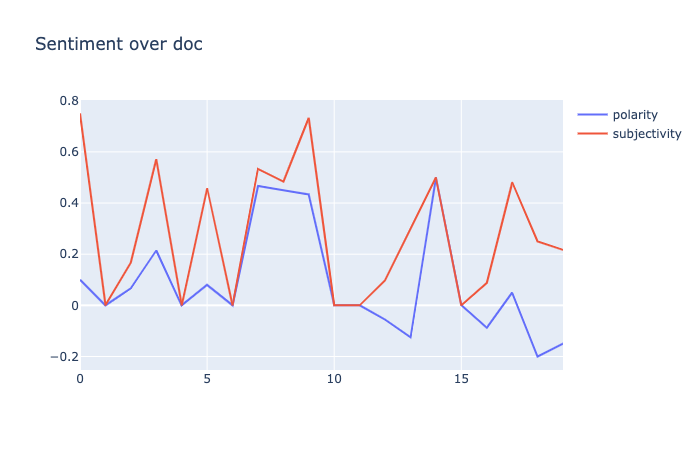
\includegraphics[width=\linewidth]{figures/sentiment_across_article.png}
    \caption{Sentiment along a single article. Each point on the x axis is a different sentence, while vertically on the y axis several scores are plotted.}
    \label{fig:sentiment_across_one_article}
\end{figure}
\todo{Fig~\ref{fig:sentiment_across_one_article} coming from which libraries?}

\subsubsection{Sentiment is correlated to citation}
By looking closely at several articles where this behaviour occurs, we noticed that this duality of tones in the articles is mostly correlated to direct/indirect reporting. When the articles give space to some interviewee (citing) the sentiment libraries detect intense and subjective words/scores. Instead, when the reporter is narrating, the tone is quieter and more neutral.

To study this correlation on large scale on our dataset, we tested our observation by automating it.
On one side, using the sentiment libraries. On the other, using a model for quotation detection~\citep{scheible2016model}.\footnote{\url{https://github.com/christianscheible/qsample}}
For each sentence, computing: sentiment score and quotation percentage (defined as number of words inside a quotation divided by total number of words).
Figure~\ref{fig:sentiment_vs_quotation} shows for the same example article, how the two are moving together.

\begin{figure}[!htbp]
    \centering
    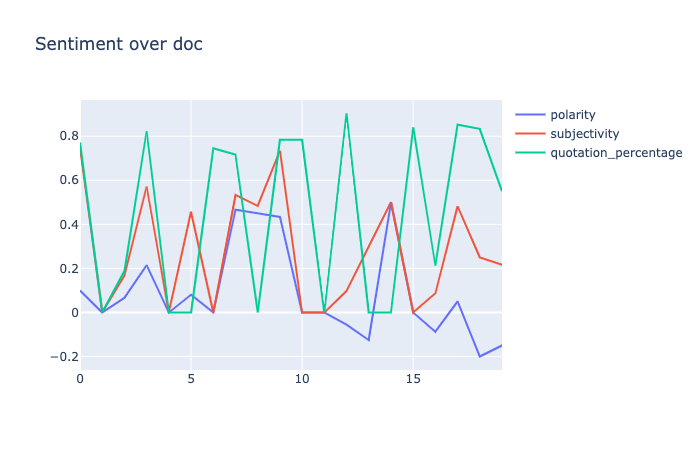
\includegraphics[width=\linewidth]{figures/sentiment_vs_quotation.png}
    \caption{Sentiment VS quotation}
    \label{fig:sentiment_vs_quotation}
\end{figure}

\todo{correlation stats across all the dataset? Quantify. Total correlation across the dataset: ??}

Finding 1:
Subjectivity and quotations: quotations increase subjectivity of articles, are the most subjective parts

Finding 2: the results of lexicon-based sentiment detection are not very great, and they are prone to many errors (e.g. Trump treated as positive words from the musical instrument).
TODO: show more qualitative analysis about this finding?w

\subsection{\statusorange Fine-grained Propaganda Analysis}

Taking from the literature described in~\ref{sec:lit_propaganda}, we consider the recent work of~\cite{da2019fine} as it is the only one that has fine-grained detection. This method uses a neural network to to annotate text articles and to see which words belong to specific propaganda techniques (Figure~\ref{fig:propaganda_example_1}).
The model is a sequence model based on BERT. It is based on the dataset CITE which contains articles annotated at the span level (specific words are highlighted and assigned to a specific technique). The model then learns to reproduce these annotations by looking at words in their context (sequence model).

It performs classification on the word level. Each word is classified as being one of 18 different techniques or none of them.

\todo{Here talk about general setup, statistics of applying propaganda detection over news articles in our datasets.}


\subsection{\statusred Propaganda vs Populism}

propaganda vs populism
\todo{this section}

Why
What
How
Results

Studying how much propaganda and populism are (correlation analysis)

dataset of populism (another one): why not the same dataset? To avoid errors on the populism detection, so that it is ground truth and errors can only be in propaganda detection.


\section{Relationship between proxies and words changed}
\label{sec:lp_relationship}

After having described in the previous sections the detection of the \emph{linguistic proxies of persuasion} on their own, we describe in this section the last stage of the pipeline announced in the introduction to this chapter (Section~\ref{sec:lp_intro}).

Therefore, here we analyse the relationship between the linguistic proxies of persuasion, and the variations across the articles (from previous Chapter~\ref{chap:common_ground_search}).

To analyse this relationship, we have two different experiments:

\begin{enumerate}
    \item variations vs propaganda: TODO
    \item improving sentence clustering by eliminating propaganda: TODO
\end{enumerate}

\subsection{\statusred Propaganda variations across similar articles}

sentiment/propaganda across related articles

Why

What

How: method

Results


Sentiment

% % sentiment
% Instead for the sentiment analysis, since we want to have detailed information (e.g. which specific words contain sentiment, and with which properties), we are relying on lexicon-based tools. Other more advanced tools (e.g. Stanford CoreNLP) have models which do not provide fine-grained scores but only sentence/document level. (This could be improved)
% % which sentiment lexicons?
% We selected some lexicons: Sentistrength, Vader, and AFINN (TODO description).
% % problems?
% The problem of doing sentiment analysis in this way is that the lexicon is recognised without accounting for other constraints (e.g. POS): we needed to remove some tools because they detected the word "Trump" as being positively loaded (trump as trumpet instead of Donald Trump).

\subsection{\statusorange Removing propaganda/sentiment to make better clustering?}

effect of sentiment/propaganda words on sentence clustering

What: removing the “highlighted” words from the article analysis, the clustering would work better or worse.

Why:
The articles are made of two components:
the story/event which can be seen from topical words, entities, …
The layer of framing which here is intended as sentiment-loaded words and propaganda techniques

Hypothesis
The framing layer does not help understanding the topics described in the articles. This set of words can be removed to perform clustering better.
We want to compare clustering of articles “as they are” and “without framing terms” and see an improvement of the clustering obtained.


How

Results

\subsubsection{Dataset}

1-Dataset: using ground truth for document clustering: so that at least we start from gold-standard groups.

As also described in the dedicated document for data, there are some datasets that we can use for having the clustering ground truth. The candidates for this experiment are:
AllSides: articles are grouped in “headlines” (3 articles for each headline) and each headline belongs to one of the 326 topics (almost all political-related). There are (updated 26th October) 5124 headlines, for a total of 15050 articles. Positive sides: human-curated, public. Negative sides: only 3 articles for each headline. But for each topic there are 46 articles on average
Google headlines: articles are grouped in clusters. Clusters have around 20-90 articles each. Each cluster belongs to a certain broader topic (UK, World, Business, Entertainment, Sports, Science, Health). Positive sides: very large. Negative side: the clusters change over time, they are created by ML (no human-curated
For this reason I initially selected AllSides.

\subsubsection{Approach}

Test the ability of matching gold clusters with predicted clusters.
- standard full article
- removing propaganda/sentiment words

Seeing if there is an improvement or not when removing propaganda words.

Removal of the terms: sentiment-loaded terms (multiple lexicons and tools: sentistrength, vader, AFINN, BING) and propaganda spans (from https://www.tanbih.org/prta).

Clustering methods:
There are multiple clustering methods, and document representations that influence the clustering. I decided to use a method that does not require to specify the number of clusters wanted.
I started with this specific method (also used in my previous analysis):
Embed the document with the Universal Sentence Encoder / TF-IDF
Use Hierarchical Agglomerative Clustering (ward method, euclidean distance), which  is very flexible in showing how the clusters evolve when the distance threshold is raised


Clustering evaluation metrics:
Although clustering is an unsupervised task, we need to see how well the clustering matches with the ground truth annotations of the data. I found online that the most used metrics for comparing clustering are:
Adjusted Rand index
Adjusted Mutual Information
The value of the metrics can be computed by comparing the ground-truth-clustering with the predicted one.
By plotting the metric values against the increasing threshold of distance of the Hierarchical Agglomerative Clustering, we can observe how it increases until a certain point, then decreases again.

TODO figure

The interpretation of this curve is that, when the hierarchical clustering begins to raise the threshold, the clusters match more with the gold clusters, until a certain point where distinct clusters are merging together and therefore lowering the scores.
We can compare the behaviour of this curve between the full text and the text without the loaded/propaganda pieces. The comparison can be at the maximum point, where the threshold is optimal (we should truncate the clustering there) or we can compare the full curve. For simplicity, in the results below, we compare the maximum value of the curve, reporting also the distance where it has been reached


\subsubsection{Findings}

Slightly easier to cluster when sentiment and propaganda words are removed from the corpus.
So propaganda and sentiment are acting like noise in clustering.

TODO explain better

